\chapter{Performance and resource usage}

This Modular Simultaneous Exponentiation IP core is designed to speed up modular simultaneous exponentiations on embedded systems.
On embedded processors, software implementations (even with specialized libraries like GMP\footnote{GNU Multiple Precision Arithmetic Library -- Project website: \url{http://gmplib.org/}}), demand much CPU time when large operands are used.
Practical tests of this core have shown a significant speed-up compared to software computations. For $n=1536$ and $t=1024$, hardware is about 70 times faster than a GMP-based implementation (with embedded linux) an a 100 MHz MicroBlaze processor (32-bit).\\

For the multiplier, execution time is given by~(\ref{eq:Tmult}), where $\tau_c$ is defined by the core operating
frequency. Since the maximum frequency is highly influenced by the latency in the critical path, we can expect to
achieve higher frequencies for shorter stage lengths. This trend is seen in Figure~\ref{fig:Virtex6exctime} for
different operand lengths, which are results used from the static timing analysis during synthesis. A minimum execution
time in this graph is found when the maximum operating frequency of the core first reaches the maximum frequency of the
FGPA in use. Beyond that point, using a smaller stage width has no positive effect anymore because the frequency can not
rise anymore and the number of clock cycles to complete a multiplication increases. Another remark that can be made is
that splitting the pipeline, has no considerable effect on the performance of the core.

\begin{figure}[H]
\centering
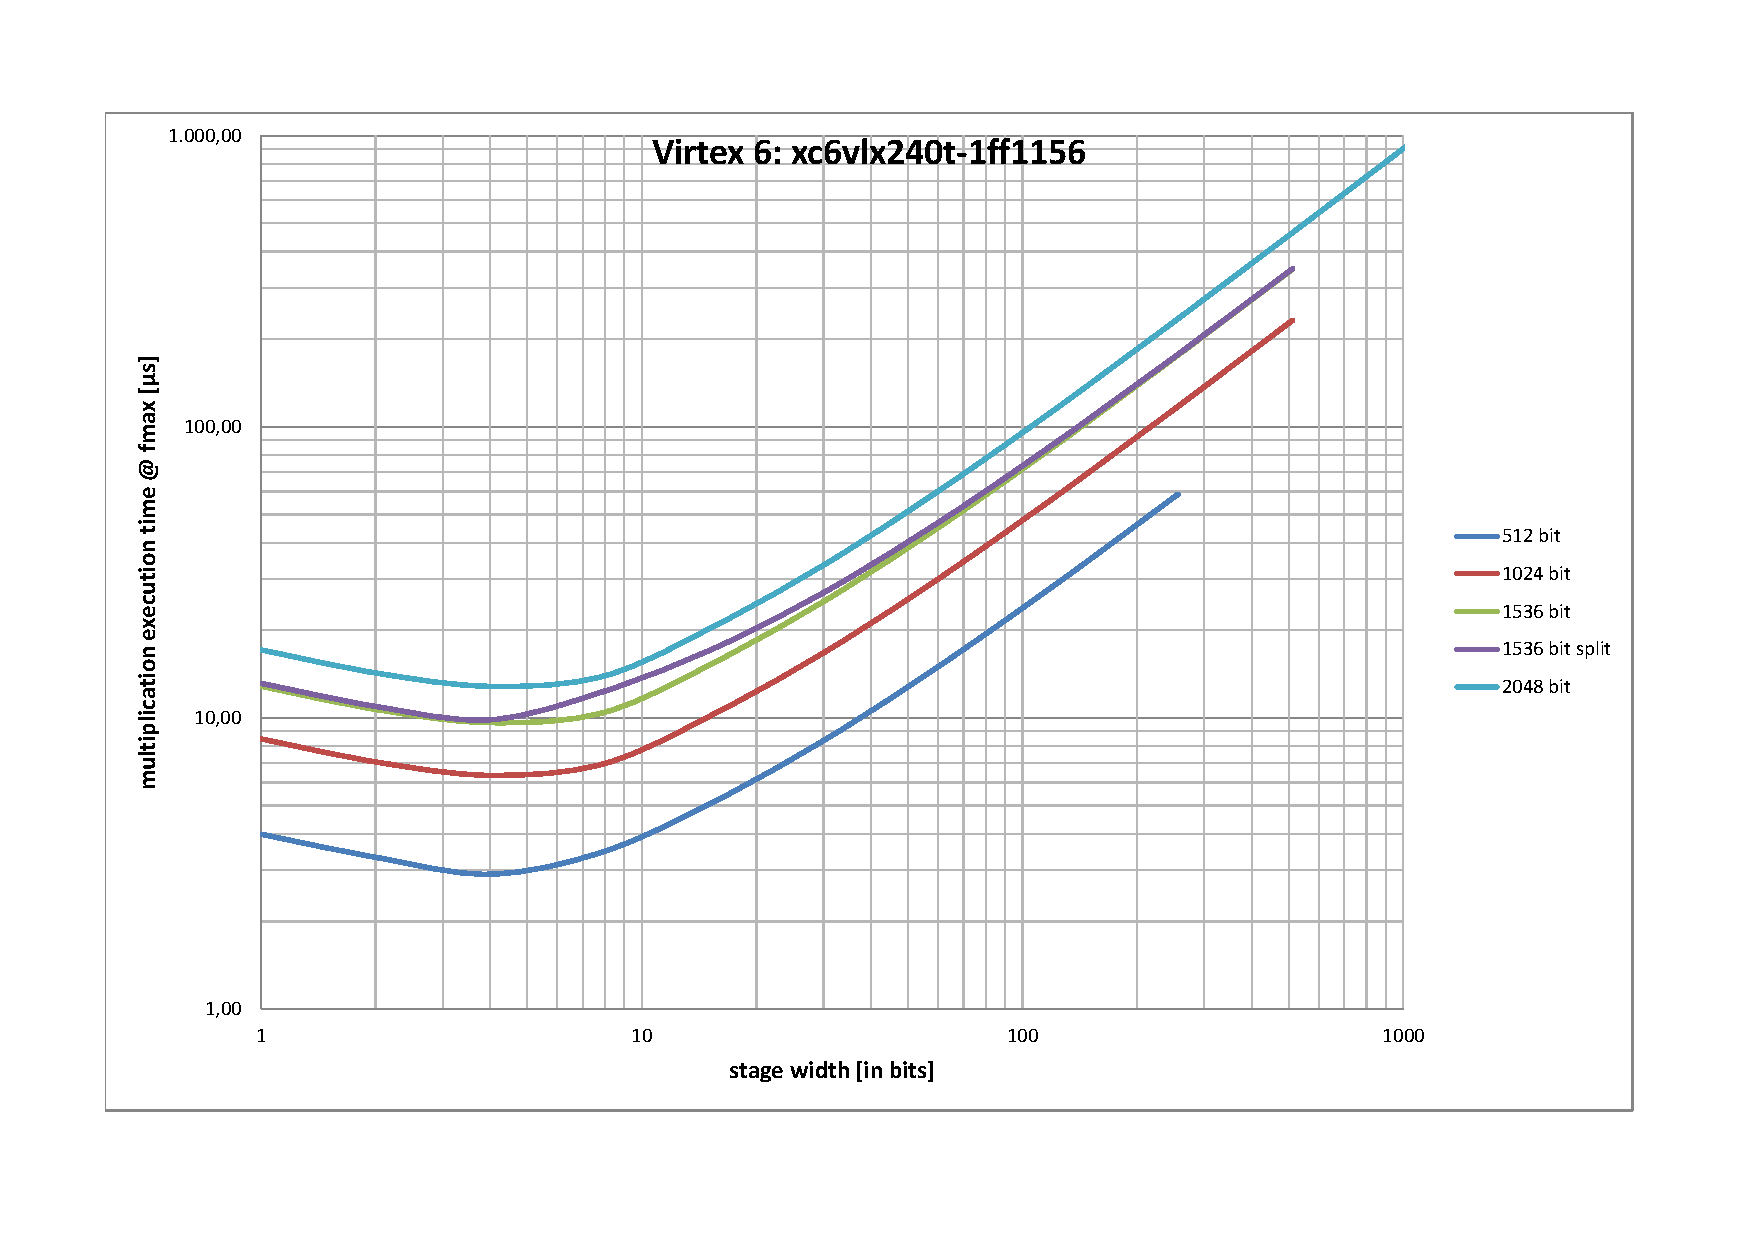
\includegraphics[trim=2cm 2cm 2cm 2cm, width=16cm]{pictures/Virtex6_stagewidth.pdf}
\caption{Example of multiplication execution time in function of the stage width for a Virtex6 FPGA.}
\label{fig:Virtex6exctime}
\end{figure}

In general, shorter stage lengths result in smaller execution times. However, using more stages implies that more
flip-flops will be needed, thus more resources are used. A balance must be found between a execution time and resources.
Currently, the core's operating frequency is the same as the bus frequency of the embedded processor. For optimal
operation of the core, the stage width must be chosen so that the maximum frequency given in synthesis is just above or
equal to the bus frequency.

In the tables below resource usage and timing results are shown for different operand lengths and FPGA's. As a rule of thumb, the number of flip-flops is given by~(\ref{eq:ff}).
\begin{align}\label{eq:ff}
5+2\cdot n+6\cdot\frac{n}{s}+\lceil\log_{2}(n)\rceil+\lceil\log_{2}(\frac{n}{s})\rceil
\end{align}
where $s$ is the stage width.

The number of LUTs is almost completely determined by $n$ and the number of LUT-inputs. A pre-synthesis estimate can be made with~(\ref{eq:lut4}) and~(\ref{eq:lut6}).
\begin{align}
8\cdot n \hspace{1cm}\text{for 4-input LUTs} \label{eq:lut4}\\
6\cdot n \hspace{1cm}\text{for 6-input LUTs} \label{eq:lut6}
\end{align}
\newline

Results for a Virtex 6 device xc6vlx240t-1ff1156, speedgrade -1\\
Synthesis settings: Optimization: area, Effort: high\\
% Table generated by Excel2LaTeX from sheet 'Virtex 6'
\begin{tabular}{rcccccccccccc}
\hline
\hline
$n$     & \multicolumn{3}{c}{512} &       & \multicolumn{3}{c}{1024} &       & \multicolumn{3}{c}{2048} & [bit] \bigstrut[t]\\
$stage width$ & 64    & 16    & 4     &       & 64    & 16    & 4     &       & 64    & 16    & 4     & [bit] \bigstrut[b]\\
\hline
$f_{max}$  & 64,91 & 199,96 & 395,57 &       & 64,91 & 199,66 & 358,62 &       & 94,91 & 199,96 & 358,62 & [MHz] \bigstrut[t]\\
$T_m@f_{max}$ & 15,87 & 5,27  & 2,91  &       & 31,77 & 10,55 & 9,63  &       & 63,57 & 21,11 & 12,84 & [$\mu$s] \\
$cycles$ & 1030  & 1054  & 1150  &       & 2062  & 2110  & 3454  &       & 4126  & 4222  & 4606  & [cycles] \\
\textbf{Resources} &       &       &       &       &       &       &       &       &       &       &       &  \\
Flipflops & 1089  & 1235  & 1813  &       & 2163  & 2453  & 5401  &       & 4309  & 4887  & 7193  &  \\
LUT's & 3094  & 3096  & 3102  &       & 6169  & 6171  & 9252  &       & 12315 & 12318 & 12324 &  \bigstrut[b]\\
\hline
\hline
\end{tabular}%
\vspace{1cm}
\newline
Results for a Spartan 3 device xc3s1000-5fg320, speedgrade -5\\
Synthesis settings: Optimization: area, Effort: high\\
% Table generated by Excel2LaTeX from sheet 'Spartan 3'
\begin{tabular}{rccccccccc}
\hline
\hline
$n$     & \multicolumn{3}{c}{256} & & \multicolumn{4}{c}{512}       & [bit] \bigstrut[t]\\
$stage width$ & 32    & 8     & 2    & & 64    & 32    & 8     & 2     & [bit] \bigstrut[b]\\
\hline
$f_max$  & 21,49 & 69,30 & 127,32 & & 11,36 & 21,49 & 69,30 & 127,32 & [MHz] \bigstrut[t]\\
$T_m@f_{max}$ & 24,1  & 7,82  & 5,01  & & 90,7  & 48,29 & 15,67 & 10,04 & [$\mu$s] \\
$cycles$ & 518   & 542   & 638 &  & 1030  & 1038  & 1086  & 1278  & [cycles] \\
\textbf{Resources} &       &    &   &       &       &       &       &       &  \\
Flipflops & 576   & 722   & 1300 & & 1089  & 1138  & 1428  & 2582  &  \\
LUT's & 2072  & 2074  & 2079 & & 4124  & 4126  & 4128  & 4135  &  \bigstrut[b]\\
\hline
\hline
\end{tabular}%
\vspace{1cm}
\newline
Results for a Virtex 4 device xc4vlx200-11ff1513, speedgrade -11\\
Synthesis settings: Optimization: area, Effort: high\\
% Table generated by Excel2LaTeX from sheet 'Virtex 4'
\begin{tabular}{rcccccccccc}
\hline
\hline
$n$     & \multicolumn{4}{c}{512}    &   & \multicolumn{4}{c}{1024}      & [bit] \bigstrut[t]\\
$stage width$ & 64    & 32    & 8     & 2    & & 128   & 32    & 8     & 2     & [bit] \bigstrut[b]\\
\hline
$f_{max}$  & 22,83 & 43,05 & 138,31 & 246,98 & & 11,77 & 43,05 & 138,31 & 246,98 & [MHz] \bigstrut[t]\\
$T_m@f_{max}$ & 45,12 & 24,11 & 7,85  & 5,17 & & 87,5  & 24,5  & 8,31  & 6,21  & [$\mu$s] \\
$cycles$ & 1030  & 1038  & 1086  & 1278 & & 1030  & 1054  & 1150  & 1534  & [cycles] \\
\textbf{Resources} &  &       &       &     &  &       &       &       &       &  \\
Flipflops & 1089  & 1138  & 1428  & 2582 & & 2114  & 2260  & 2838  & 5144  &  \\
LUT's & 4124  & 4126  & 4128  & 4135 & & 8225  & 8230  & 8234  & 8238  &  \bigstrut[b]\\
\hline
\hline
\end{tabular}%

